\documentclass[../main.tex]{subfiles}

\begin{document}

\section{Results}

\subsection{Cluster Sizing using Image Processing}

The following section contains results from image processing based techniques as described in section~\ref{sec:methods:imageprocessing}.

\subsubsection{Epifluorescence Microscopy}

These experiments were performed on a Nikon microscope on loan from the manufacturer. One image was taken each from a slide of cells prepared with and without cobalt.

\begin{figure}[h!]
\begin{center}
\subfigure[No cobalt, \(n=18, \mu=0.144, \sigma=0.070\)]{
	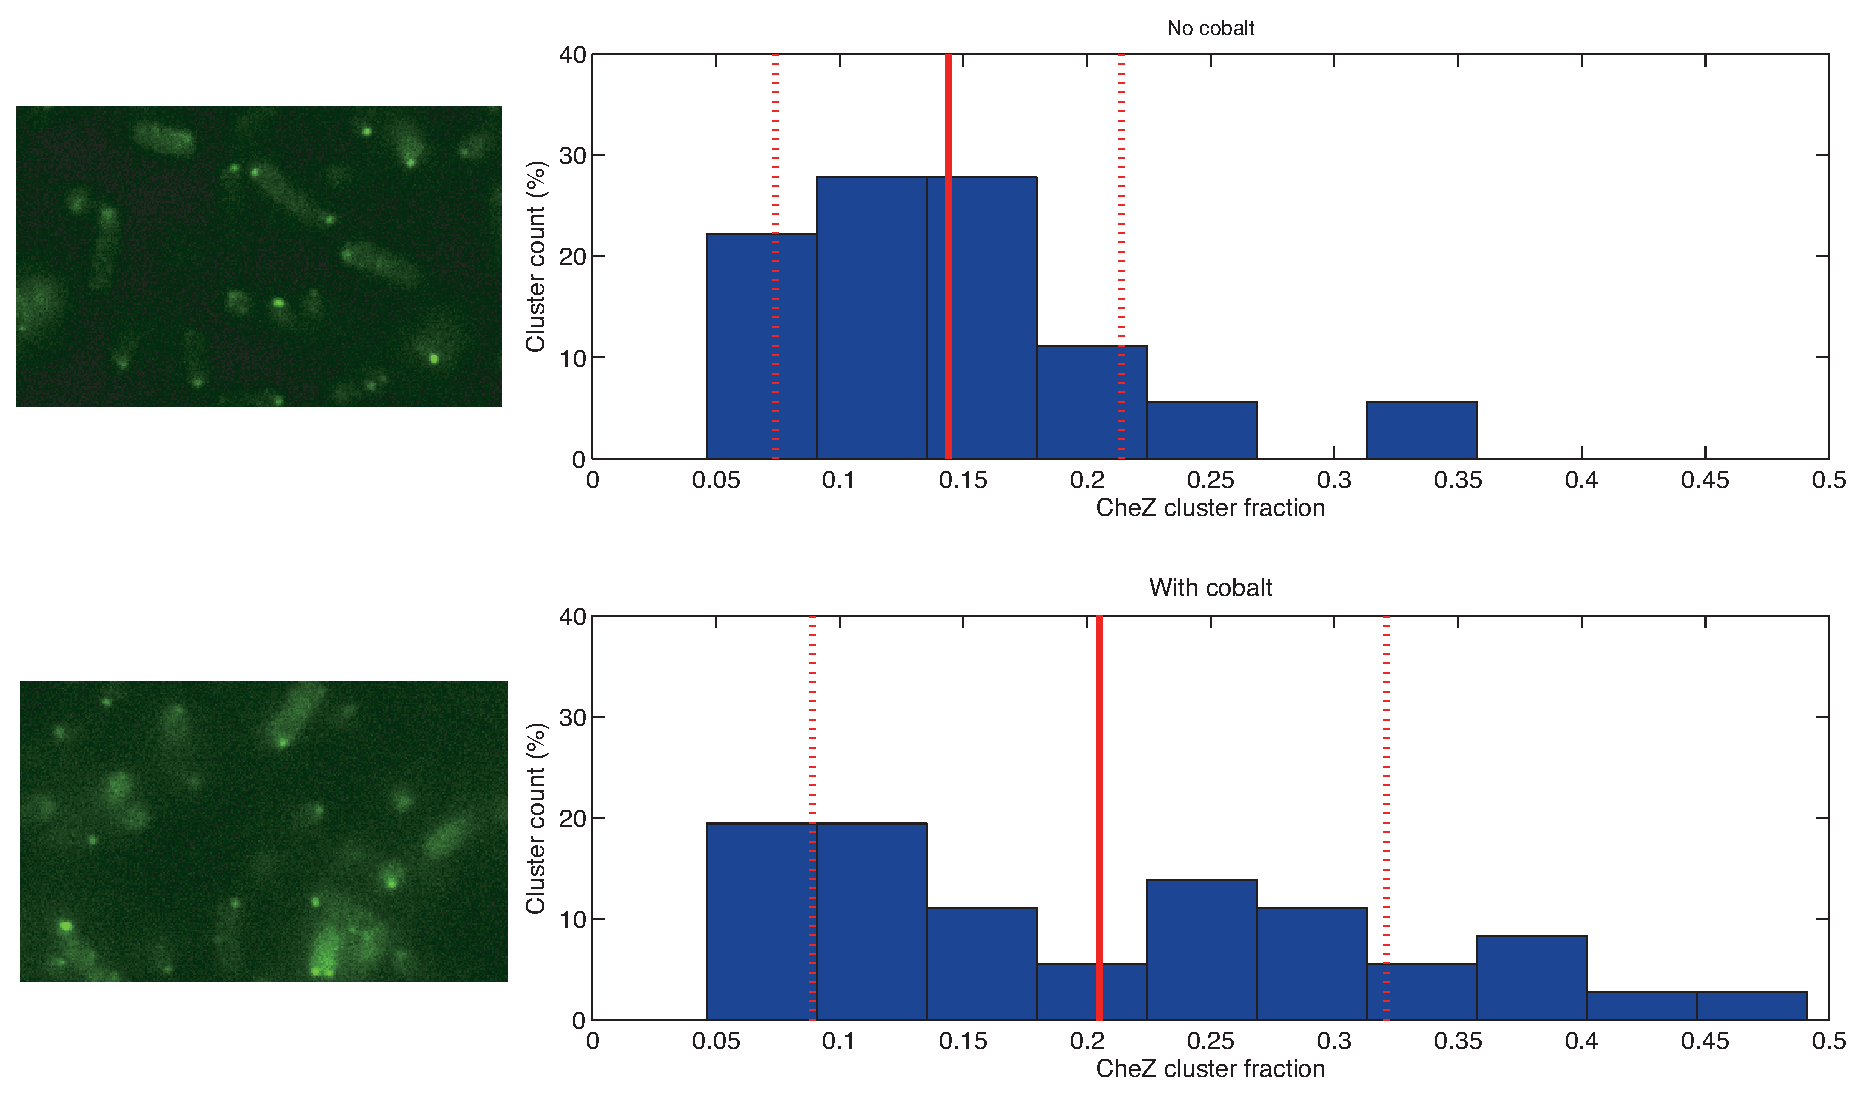
\includegraphics[scale=0.65, trim=0 300 0 40, clip=true]{\docroot results/figs/nikonb.eps}
	\label{fig:results:nikon:nocobalt}
}\\
\subfigure[With cobalt, \(n=36, \mu=0.205, \sigma=0.116\)]{
	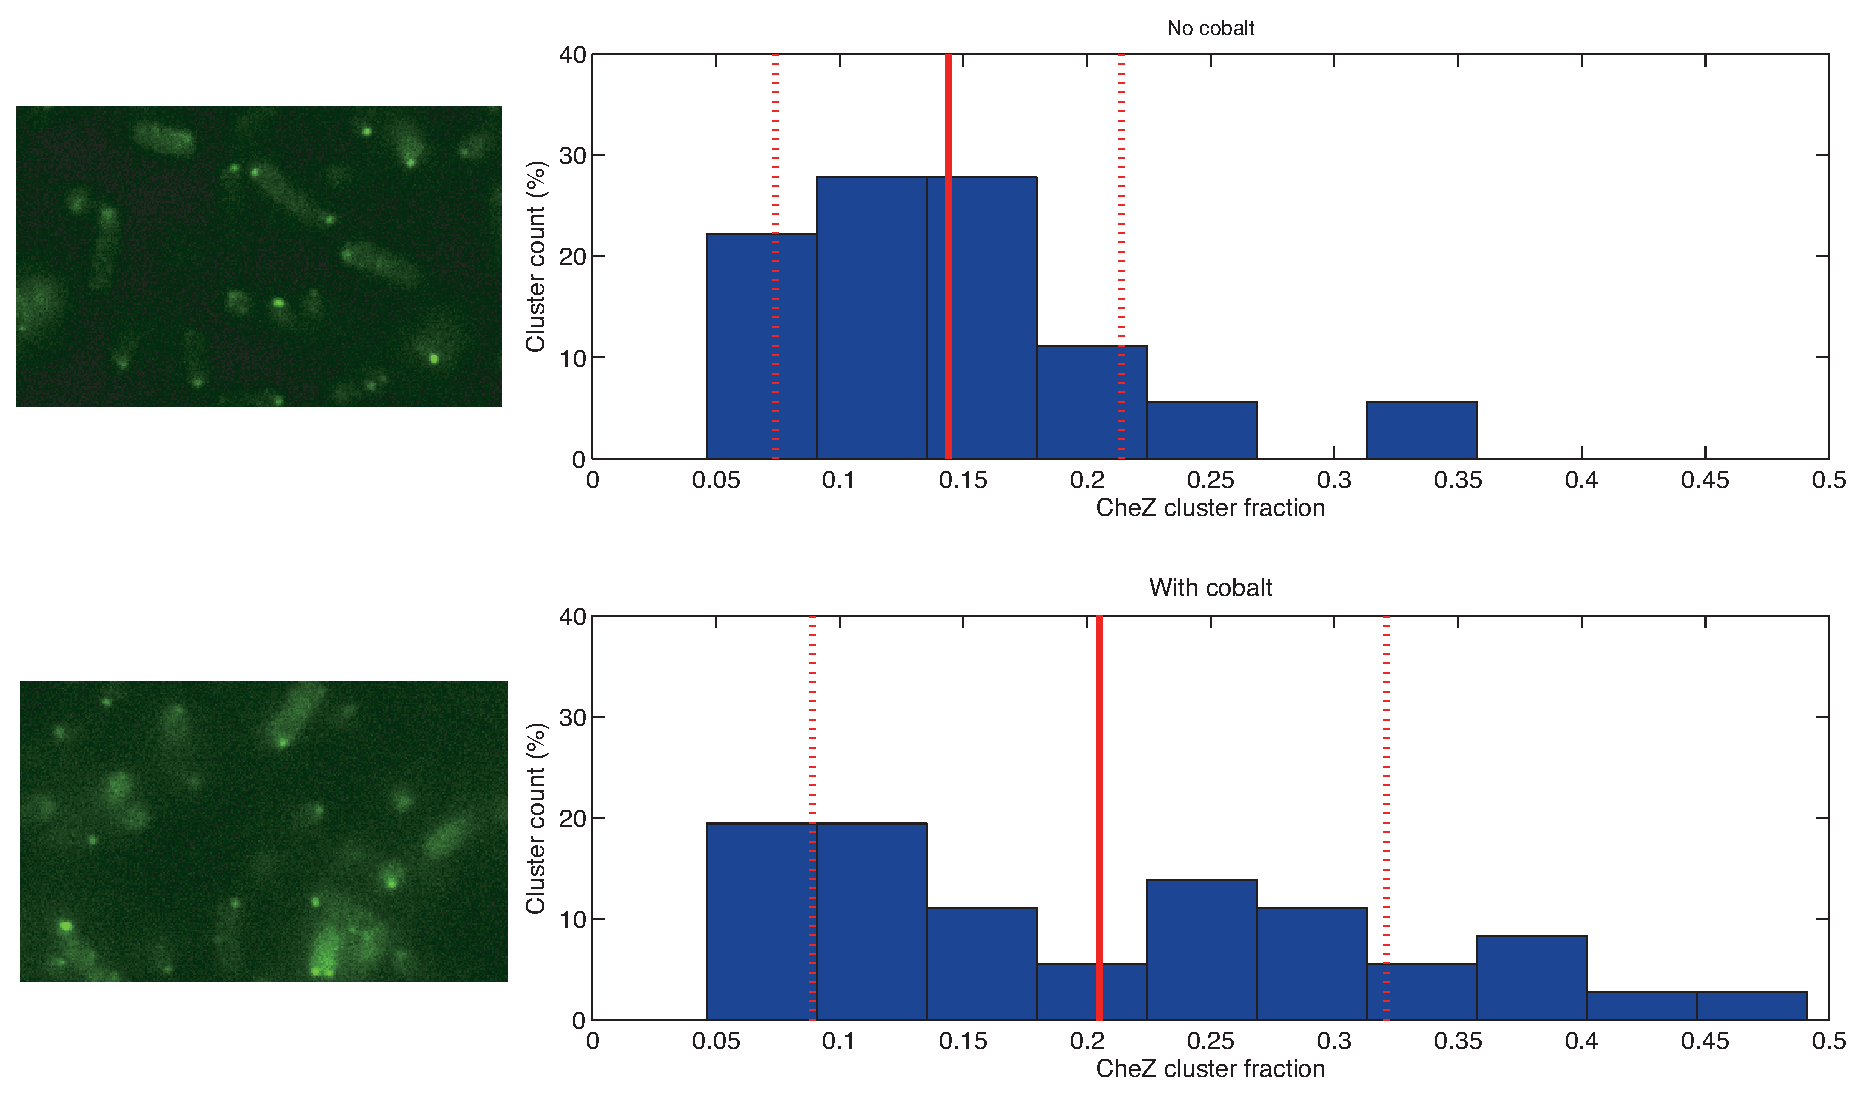
\includegraphics[scale=0.65, trim=0 30 0 310, clip=true]{\docroot results/figs/nikonb.eps}
	\label{fig:results:nikon:cobalt}
}
\caption{Histograms of CheZ cluster fraction (fraction of CheZ protein in cell localised in the polar cluster). Solid red line marks mean average, dashed lines \(\pm\sigma\).}
\label{fig:results:nikon}
\end{center}
\end{figure}

\subsubsection{Confocal Microscopy}

These experiments were performed on a Zeiss confocal microscope, the use of which was kindly given to us by Alessandro Esposito at the Hutchison MRC. Ten images were taken each from a slide of cells prepared with and without cobalt.

\begin{figure}[h!]
\begin{center}
\subfigure[No cobalt, \(n=1222, \mu=0.185, \sigma=0.068\)]{
	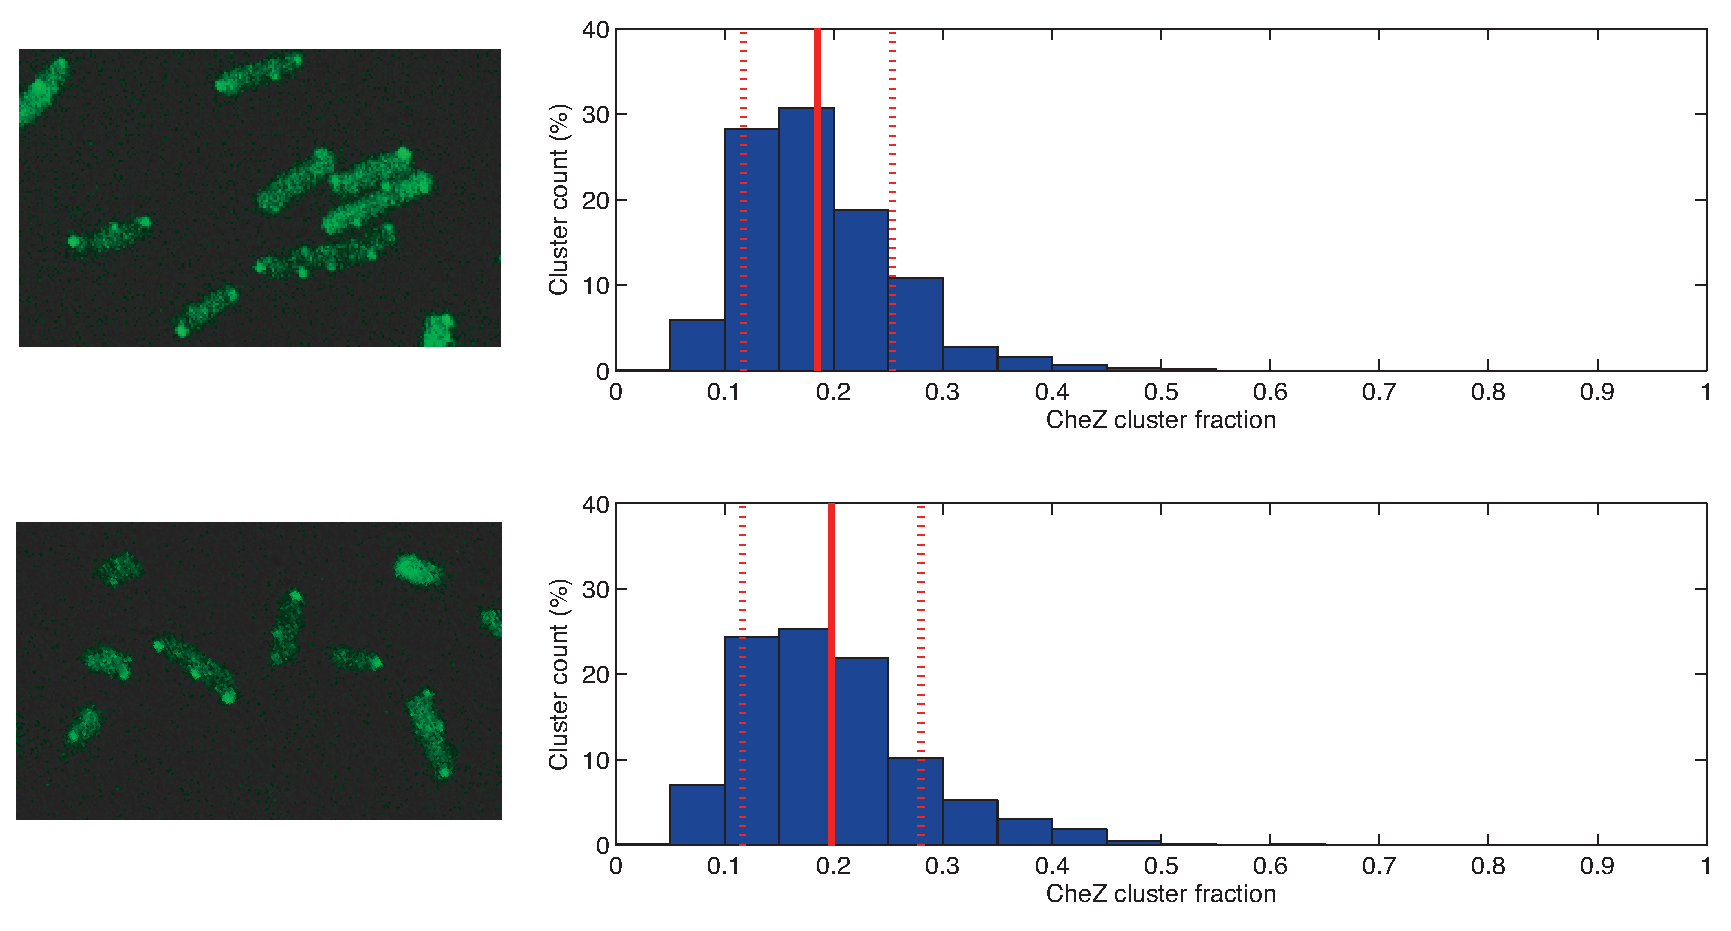
\includegraphics[scale=0.65, trim=0 250 0 30, clip=true]{\docroot results/figs/zeiss.eps}
	\label{fig:results:zeiss:nocobalt}
}\\
\subfigure[With cobalt, \(n=644, \mu=0.198, \sigma=0.082\)]{
	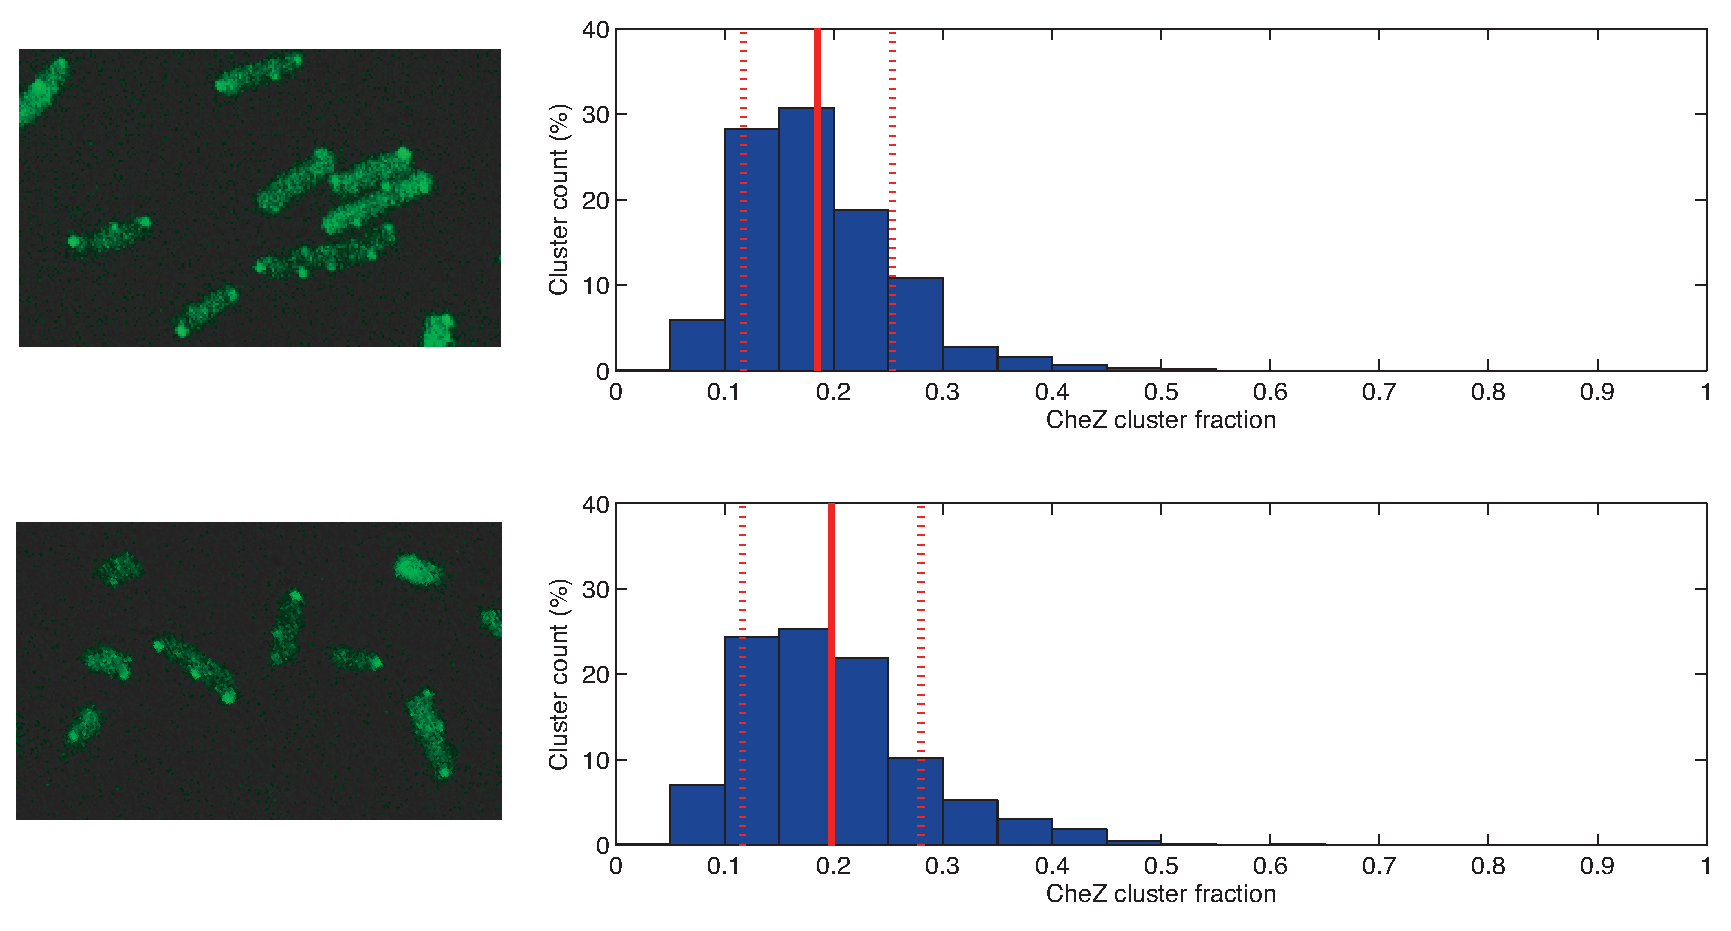
\includegraphics[scale=0.65, trim=0 20 0 260, clip=true]{\docroot results/figs/zeiss.eps}
	\label{fig:results:zeiss:cobalt}
}
\caption{Histograms of CheZ cluster fraction (fraction of CheZ protein in cell localised in the polar cluster). Solid red line marks mean average, dashed lines \(\pm\sigma\). \(p\) value \(=0.0349\%\).}
\label{fig:results:zeiss}
\end{center}
\end{figure}

\begin{comment}
\subsection{Inducer Calibration}

\paragraph{Inducement Time}

\begin{table}[h!]
\begin{center}
\begin{tabular}{l|c|c|c|c|c|c}
\multirow{2}{*}{\textbf{Time}} &	\multicolumn{3}{c|}{\textbf{Induced t=0}}  &	\multicolumn{3}{c}{\textbf{Induced t=2}}	\\
& \textbf{A} & \textbf{E} & \textbf{S} & \textbf{A} & \textbf{E} & \textbf{S} \\\hline
Overnight Culture & 0.321 & 0.295 & 0.300 & 0.312 & 0.295 & 0.300\\
\SI{2}{\hour} & 0.026 & 0.032 & 0.050 & 0.029 & 0.031 & 0.040
\end{tabular}
\end{center}
\end{table}
\end{comment}

\end{document}